\documentclass[a4paper,14pt]{article}

%%% Работа с русским языком
\usepackage{cmap}					% поиск в PDF
\usepackage{mathtext} 				% русские буквы в формулах
\usepackage[T2A]{fontenc}			% кодировка
\usepackage[utf8]{inputenc}			% кодировка исходного текста
\usepackage[english,russian]{babel}	% локализация и переносы
\usepackage{indentfirst}
\frenchspacing

\newcommand{\vyp}{\ensuremath{\hookrightarrow}}
\renewcommand{\epsilon}{\ensuremath{\varepsilon}}
\renewcommand{\phi}{\ensuremath{\varphi}}
\renewcommand{\kappa}{\ensuremath{\varkappa}}
\renewcommand{\le}{\ensuremath{\leqslant}}
\renewcommand{\leq}{\ensuremath{\leqslant}}
\renewcommand{\ge}{\ensuremath{\geqslant}}
\renewcommand{\geq}{\ensuremath{\geqslant}}
\renewcommand{\emptyset}{\varnothing}
\newcommand{\Ra}{\ensuremath{\Rightarrow}}
\newcommand{\ra}{\ensuremath{\rightarrow}}
\newcommand{\LRa}{\ensuremath{\Leftrightarrow}}
\newcommand{\tbf}{\textbf}
\newcommand{\ov}{\ensuremath{\overline}}
\newcommand{\CC}{\ensuremath{\mathbb{C}}}
\newcommand{\RR}{\ensuremath{\mathbb{R}}}
\newcommand{\NN}{\ensuremath{\mathbb{N}}}
\newcommand{\QQ}{\ensuremath{\mathbb{Q}}}
\newcommand{\ZZ}{\ensuremath{\mathbb{Z}}}

%%% Дополнительная работа с математикой
\usepackage{amsmath,amsfonts,amssymb,amsthm,mathtools} % AMS
\usepackage{icomma} % "Умная" запятая: $0,2$ --- число, $0, 2$ --- перечисление

%% Номера формул
%\mathtoolsset{showonlyrefs=true} % Показывать номера только у тех формул, на которые есть \eqref{} в тексте.
%\usepackage{leqno} % Нумереация формул слева

%% Свои команды
\DeclareMathOperator{\sgn}{\mathop{sgn}}

%% Перенос знаков в формулах (по Львовскому)
\newcommand*{\hm}[1]{#1\nobreak\discretionary{}
{\hbox{$\mathsurround=0pt #1$}}{}}



%%% Работа с картинками
\usepackage{graphicx}  % Для вставки рисунков
\graphicspath{{images/}{images2/}}  % папки с картинками
\setlength\fboxsep{3pt} % Отступ рамки \fbox{} от рисунка
\setlength\fboxrule{1pt} % Толщина линий рамки \fbox{}
\usepackage{wrapfig} % Обтекание рисунков текстом

%%% Работа с таблицами
\usepackage{array,tabularx,tabulary,booktabs} % Дополнительная работа с таблицами
\usepackage{longtable}  % Длинные таблицы
\usepackage{multirow} % Слияние строк в таблице

%%% Теоремы
\theoremstyle{plain} % Это стиль по умолчанию, его можно не переопределять.
\newtheorem{theorem}{Теорема}[section]
\newtheorem{proposition}[theorem]{Утверждение}
 
\theoremstyle{definition} % "Определение"
\newtheorem{corollary}{Следствие}[theorem]
\newtheorem{problem}{Задача}[section]
 
\theoremstyle{remark} % "Примечание"
\newtheorem*{nonum}{Решение}

%%% Программирование
\usepackage{etoolbox} % логические операторы

%%% Страница
\usepackage{extsizes} % Возможность сделать 14-й шрифт
\usepackage{geometry} % Простой способ задавать поля
	\geometry{top=20mm}
	\geometry{bottom=20mm}
	\geometry{left=5mm}
	\geometry{right=15mm}
 %
\usepackage{fancyhdr} % Колонтитулы
 	\pagestyle{fancy}
 	\renewcommand{\headrulewidth}{1pt}  % Толщина линейки, отчеркивающей верхний колонтитул
%\fancypagestyle{firstpage}{
	\rhead{\large{Исыпов Илья}}
%}
% 	\lfoot{Нижний левый}
% 	\rfoot{\large{Рябых Владислав, Б05-905}}
% 	\rhead{Верхний правый]}
% 	\chead{Верхний в центре}
 	\lhead{\large{Рябых Владислав}}
%	\cfoot{Нижний в центре} % По умолчанию здесь номер страницы

\usepackage{setspace} % Интерлиньяж
\onehalfspacing % Интерлиньяж 1.5
%\doublespacing % Интерлиньяж 2
%\singlespacing % Интерлиньяж 1

\usepackage{lastpage} % Узнать, сколько всего страниц в документе.

\usepackage{soul} % Модификаторы начертания

\usepackage{hyperref}
\usepackage[usenames,dvipsnames,svgnames,table,rgb]{xcolor}
\hypersetup{				% Гиперссылки
    unicode=true,           % русские буквы в раздела PDF
    pdftitle={Заголовок},   % Заголовок
    pdfauthor={Автор},      % Автор
    pdfsubject={Тема},      % Тема
    pdfcreator={Создатель}, % Создатель
    pdfproducer={Производитель}, % Производитель
    pdfkeywords={keyword1} {key2} {key3}, % Ключевые слова
    colorlinks=true,       	% false: ссылки в рамках; true: цветные ссылки
    linkcolor=red,          % внутренние ссылки
    citecolor=black,        % на библиографию
    filecolor=magenta,      % на файлы
    urlcolor=cyan           % на URL
}

\usepackage{csquotes} % Еще инструменты для ссылок

%\usepackage[style=authoryear,maxcitenames=2,backend=biber,sorting=nty]{biblatex}

\usepackage{multicol} % Несколько колонок

\usepackage{tikz} % Работа с графикой
\usepackage{pgfplots}
\usepackage{pgfplotstable}

\usepackage{caption}
\long\def\comment{}
\setlength{\abovecaptionskip}{7pt}
\setlength{\belowcaptionskip}{7pt}
\usepackage {upgreek}


\begin{document}
\author{Рябых Владислав и Исыпов Илья, Б05-905}
\title{\tbf{3.4.4 (128). Петля гистерезиса (статический метод)}}
\maketitle

\tbf{Цель работы:} наблюдение начальной кривой намагничивания ферромагнетиков и предельной петли гистерезиса.

\tbf{В работе используются:} источник питания, тороид, соленоид, баллистический гальванометр с осветителем и шкалой, амперметр, магазин сопротивлений, лабораторный автотрансформатор (ЛАТР), разделительный трансформатор.


\section*{Теория}
Магнитная индукция $B$ и напряженность магнитного поля $H$ в ферромагнетиках связаны между собой сложным нелинейным образом: индукция зависит не только от напряженности, но и от предыстории образца. Связь между $B$ и $H$ типичного ферромагнетика иллюстрирует рис. \ref{pic1}. Выходящая из начала координат основная кривая намагничивания $OACD$ возникает при намагничивании размагниченного образца.

\begin{center}
\begin{figure}[bhtp]
	\centering
	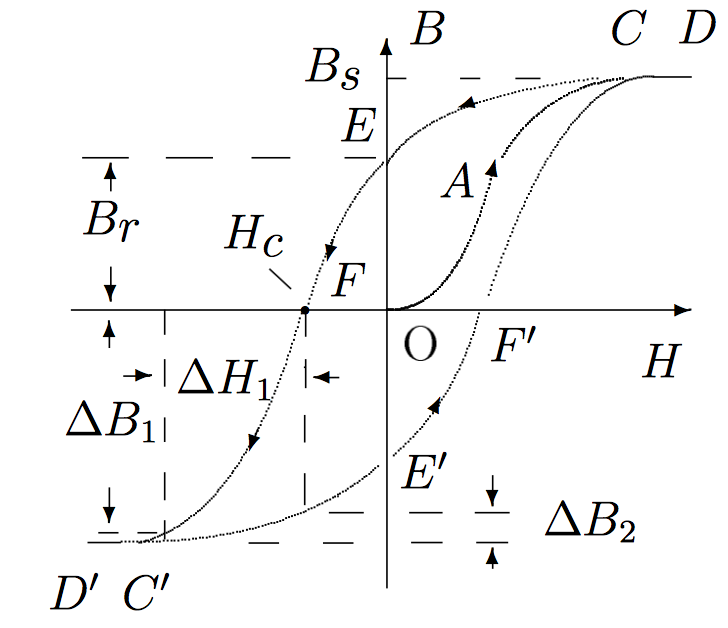
\includegraphics[width=0.32\linewidth]{pic1.png}
	\caption{петля гистерезиса ферромагнетика}
	\label{pic1}
\end{figure}
\end{center}

Зададимся целью определить коэрцитивную силу и индукцию насыщения предоставленного образца (материал ~--- сталь).
Индукция в образце складывается из напряжённости внешнего поля $H$ и намагниченности образца: 
$B = \mu_0 (H + M)$, где намагниченность $M$ ~--- магнитный момент единицы объема образца, а $\mu_0$ ~--- магнитная постоянная.

Сначала намагнитим образец до насыщения (точка $D$). Соответствующее значение индукции $B_s$ называют индукцией насыщения. Потом будем постепенно уменьшать внешнее поле. Явление гистерезиса состоит в том, что при нулевом значении внешнего поля индукция остаётся некоторая остаточная индукция ~$B_r$. Чтобы размагнитить образец, то есть перевести его в состояние $F$, необходимо приложить «обратное» магнитное поле~$-H_c$, которое называют коэрцитивной силой.
Замкнутая кривая $DEFD'E'F'D$, возникающая при циклическом перемагничивании образца, намагниченного до насыщения, называется предельной петлёй гистерезиса.


Необходимо выразить $H$ и $B$ через параметры, измеряемые в эксперименте.
Напряженность магнитного поля в $H$ в тороиде зависит от тока, текущего в обмотке: 

\begin{equation}
H \approx \dfrac{N}{\pi D} I
\label{eqH}
\end{equation}
где $D$~--- средний диаметр тора, $N$~--- число витков.

При скачкообразном изменении тока на величину $\Delta I$ поле в тороиде меняется: $\Delta H \sim \Delta I$. Изменение $\Delta H$ приводит к изменению потока магнитной индукции $\Phi$ в сердечнике, и в измерительной обмотке сечения $S_T$ с числом витков $N_{T1}$ возникает ЭДС индукции:
$$ \mathcal{E} = - \dfrac{d \Phi}{dt} = - S N' \dfrac{dB}{dt}.$$

Через гальванометр протекает импульс тока; первый отброс зайчика гальванометра, работающего в баллистическом режиме, пропорционален величине прошедшего через гальванометр заряда $q$:
$$\varphi = \dfrac{q}{b},$$
где $b$~--- баллистическая постоянная гальванометра. 

Дополнительно для получения баллистической постоянной необходимо использовать вместо тороида пустотелый соленоид с числом витков $N_{T0}$, с $N_{T1}$ витками на измерительной катушке, длиной $l_c$. Тогда исключив баллистическую постоянную и выразив $\Delta B$ получим выражение: 
\begin{equation}
	\Delta B  = \mu_0 N_c \dfrac{N_c'}{N'} \left( \dfrac{d_C}{d} \right)^2 \dfrac{R}{R_c} \dfrac{N_{C0}}{N_{T1}} \dfrac{\Delta I_c}{l_c} \dfrac{\Delta x}{\Delta x_c}.
	\label{eq1}
\end{equation}

Измерение предельной петли гистерезиса начинаем с максимального значения магнитного поля, что соответствует точке $D$ на рис. \ref{pic1}. Специальный генератор позволяет скачками менять токи в намагничивающей обмотке. Он работает неравномерно, так как разные скачки на разных участках петли вызывают разные отклонения зайчика гальванометра (большие скачки делаются вблизи насыщения и малые вблизи нуля). Дойдя до нулевого значения тока ($E$), меняем направление магнитного поля и снова увеличиваем ток в намагничивающей обмотке ($D'$). Затем снова меняем направление магнитного поля и возвращаемся в точку $D$.

Сопротивления измерительных цепей $R$ и $R_1$ подбираются одинаковыми, чтобы можно было считать постоянную гальванометра действительно постоянной (в общем случае она зависит от полного сопротивления в цепи).

Измерение начальной кривой намагничивания (участок $OAC$) производится по той же схеме, но с предварительно размагниченным образцом. 

\section*{Экспериментальная установка}

\begin{center}
\begin{figure}[bhtp]
	\centering
	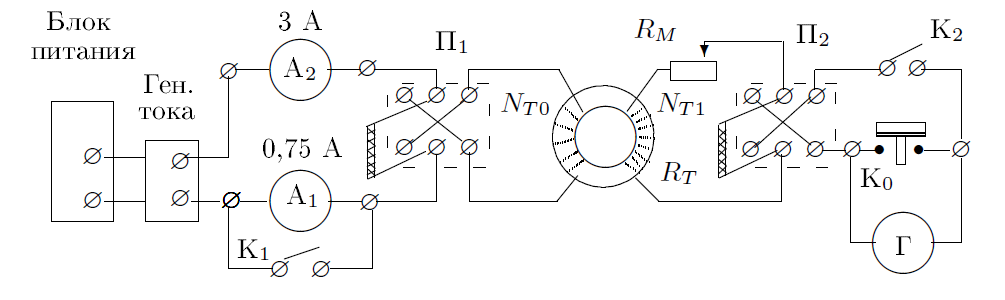
\includegraphics[width=\linewidth]{scheme1.png}
	\caption{схема установки для исследования петли гистерезиса}
	\label{scheme1}
\end{figure}
\end{center}

После снятия петли гистерезиса необходимо размагнитить сердечник, подключив его к цепи переменного тока, постепенно снижая его амплитуду. Только затем следует приступать к снятию основной кривой намагничивания.

\begin{center}
\begin{figure}[bhtp]
\centering
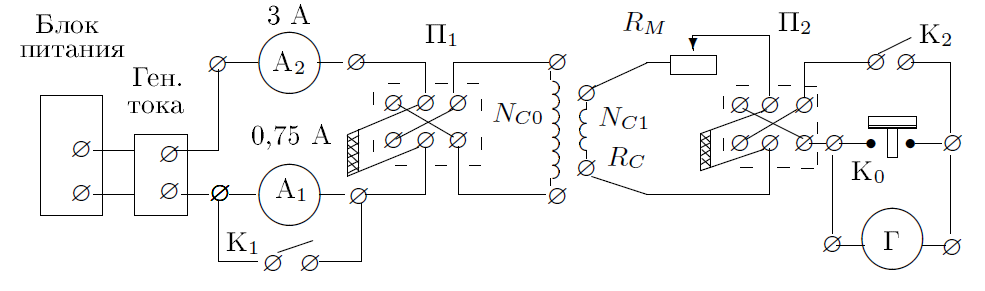
\includegraphics[width=\linewidth]{scheme2.png}
\caption{схема установки для калибровки гальванометра}
\label{scheme2}
\end{figure}
\end{center}


\section*{Ход работы}
Подготовив к работе экспериментальную установку по схеме 1 с рис. \ref{scheme1}, $R_\text{м}$ = 140 Ом. Снимем зависимость величины скачка зайчика $\Delta x$ от величины силы тока в цепи $I$. $H$ вычисляем по формуле \eqref{eqH}. Результаты измерений приведены в таблицах \ref{tabb} и \ref{tabb2}.

\begin{table}[hbt!]
	\begin{center}
	\begin{tabular}{|c|c|c|c|c|c|}
		\hline
		состояние кнопки & $I$, А     & $H$, A/м        & $\Delta x$, см & $\Delta B$, Tл & $B$, Tл \\ \hline
15               & 1.70   & 306.0   &             &             &       \\ \hline
14               & 1.20   & 216.0   & 2.9         & 0.11        & 0.1   \\ \hline
13               & 0.87   & 156.6   & 2.7         & 0.10        & 0.2   \\ \hline
12               & 0.62   & 111.6   & 2.7         & 0.10        & 0.3   \\ \hline
11               & 0.43   & 77.4    & 2.6         & 0.10        & 0.4   \\ \hline
10               & 0.35   & 63.0    & 1.4         & 0.05        & 0.5   \\ \hline
9                & 0.30   & 54.0    & 0.8         & 0.03        & 0.5   \\ \hline
8                & 0.27   & 48.6    & 0.5         & 0.02        & 0.5   \\ \hline
7                & 0.25   & 45.0    & 0.4         & 0.02        & 0.5   \\ \hline
6                & 0.23   & 41.4    & 0.4         & 0.02        & 0.6   \\ \hline
5                & 0.21   & 37.8    & 0.4         & 0.02        & 0.6   \\ \hline
4                & 0.19   & 34.2    & 0.5         & 0.02        & 0.6   \\ \hline
3                & 0.17   & 30.6    & 0.5         & 0.02        & 0.6   \\ \hline
2                & 0.12   & 21.6    & 1.2         & 0.05        & 0.7   \\ \hline
1                & 0.06   & 10.8    & 1.6         & 0.06        & 0.7   \\ \hline
0                & 0.00   & 0.0     & 1.9         & 0.07        & 0.8   \\ \hline
1                & -0.06  & -10.8   & 2.2         & 0.08        & 0.9   \\ \hline
2                & -0.12  & -21.6   & 2.9         & 0.11        & 1.0   \\ \hline
3                & -0.17  & -30.6   & 3.5         & 0.13        & 1.1   \\ \hline
4                & -0.19  & -34.2   & 1.9         & 0.07        & 1.2   \\ \hline
5                & -0.21  & -37.8   & 2.4         & 0.09        & 1.3   \\ \hline
6                & -0.23  & -41.4   & 2.8         & 0.11        & 1.4   \\ \hline
7                & -0.25  & -45.0   & 3.6         & 0.14        & 1.5   \\ \hline
8                & -0.27  & -48.6   & 4.6         & 0.18        & 1.7   \\ \hline
9                & -0.30  & -54.0   & 6.8         & 0.26        & 2.0   \\ \hline
10               & -0.35  & -63.0   & 10.4        & 0.40        & 2.4   \\ \hline
11               & -0.43  & -77.4   & 12.9        & 0.50        & 2.9   \\ \hline
12               & -0.62  & -111.6  & 12.0        & 0.46        & 3.3   \\ \hline
13               & -0.87  & -156.6  & 7.0         & 0.27        & 3.6   \\ \hline
14               & -1.20  & -216.0  & 5.1         & 0.20        & 3.8   \\ \hline
15               & -1.70  & -306.0  & 4.4         & 0.17        & 4.0   \\ \hline
	\end{tabular}
\caption{результаты измерений}
\label{tabb}
\end{center}
\end{table}

\clearpage

\begin{table}[hbt!]
	\begin{center}
		\begin{tabular}{|c|c|c|c|c|c|}
			\hline
			состояние кнопки & $I$, А     & $H$, A/м          & $\Delta x$, см & $\Delta B$, Tл & $B$, Tл \\ \hline
15               & -1.70  & -306.0  & 4.4         & 0.17        & 4.0   \\ \hline
14               & -1.20  & -216.0  & 2.9         & 0.11        & 3.9   \\ \hline
13               & -0.87  & -156.6  & 2.7         & 0.10        & 3.7   \\ \hline
12               & -0.62  & -111.6  & 2.7         & 0.10        & 3.6   \\ \hline
11               & -0.43  & -77.4   & 2.6         & 0.10        & 3.5   \\ \hline
10               & -0.35  & -63.0   & 1.4         & 0.05        & 3.5   \\ \hline
9                & -0.30  & -54.0   & 0.8         & 0.03        & 3.5   \\ \hline
8                & -0.27  & -48.6   & 0.5         & 0.02        & 3.4   \\ \hline
7                & -0.25  & -45.0   & 0.4         & 0.02        & 3.4   \\ \hline
6                & -0.23  & -41.4   & 0.5         & 0.02        & 3.4   \\ \hline
5                & -0.21  & -37.8   & 0.4         & 0.02        & 3.4   \\ \hline
4                & -0.19  & -34.2   & 0.5         & 0.02        & 3.4   \\ \hline
3                & -0.17  & -30.6   & 0.5         & 0.02        & 3.4   \\ \hline
2                & -0.12  & -21.6   & 1.2         & 0.05        & 3.3   \\ \hline
1                & -0.06  & -10.8   & 1.6         & 0.06        & 3.2   \\ \hline
0                & 0.00   & 0.0     & 1.8         & 0.07        & 3.2   \\ \hline
1                & 0.06   & 10.8    & 2.2         & 0.08        & 3.1   \\ \hline
2                & 0.12   & 21.6    & 2.9         & 0.11        & 3.0   \\ \hline
3                & 0.17   & 30.6    & 3.5         & 0.13        & 2.8   \\ \hline
4                & 0.19   & 34.2    & 2.0         & 0.08        & 2.8   \\ \hline
5                & 0.21   & 37.8    & 2.4         & 0.09        & 2.7   \\ \hline
6                & 0.23   & 41.4    & 2.8         & 0.11        & 2.6   \\ \hline
7                & 0.25   & 45.0    & 3.6         & 0.14        & 2.4   \\ \hline
8                & 0.27   & 48.6    & 4.6         & 0.18        & 2.3   \\ \hline
9                & 0.30   & 54.0    & 6.9         & 0.27        & 2.0   \\ \hline
10               & 0.35   & 63.0    & 10.5        & 0.40        & 1.6   \\ \hline
11               & 0.43   & 77.4    & 12.6        & 0.48        & 1.1   \\ \hline
12               & 0.62   & 111.6   & 12.0        & 0.46        & 0.6   \\ \hline
13               & 0.87   & 156.6   & 7.1         & 0.27        & 0.4   \\ \hline
14               & 1.20   & 216.0   & 5.1         & 0.20        & 0.2   \\ \hline
15               & 1.70   & 306.0   & 4.3         & 0.17        & 0.0   \\ \hline
	\end{tabular}
\caption{результаты измерений}
\label{tabb2}
\end{center}
\end{table}
\clearpage

Для калибровки гальваноида подключим соленоид по схеме на рис. \ref{scheme2}. Уменьшим сопротивление магазина $R_\text{м}$ на величину $R_\text{с} = 46$ Ом: $R_\text{м} = 140 - 46 = 94$ Ом. Получим следующие значения для тока и максимального отклонения:
\[
\Delta x_c = 23.5 \ \text{см}, \ \Delta I_c = 1.70 \ \text{А}
\]

После этого отключаем соленоид, собираем схему 1 на рис. \ref{scheme1}, возвращаем магазину начальное сопротивление $R_\text{м}$ = 140 Ом и проведём снятие начальной кривой намагничивания для размагниченного образца. Результаты измерений приведены в таблице \ref{namagn}.

\begin{table}[hbt!]
\begin{center}
\begin{tabular}{|c|c|c|c|c|c|}
	\hline
	состояние кнопки & $I$, А     & $H$, A/м          & $\Delta x$, см & $\Delta B$, Tл & $B$, Tл \\ \hline
	0                & 0.00 & 0.0   &             &              &     \\ \hline
	1                & 0.06 & 10.8  & 3.3         & 0.04         & 0.0 \\ \hline
	2                & 0.12 & 21.6  & 6.1         & 0.08         & 0.1 \\ \hline
	3                & 0.17 & 30.6  & 6.7         & 0.09         & 0.2 \\ \hline
	4                & 0.19 & 34.2  & 2.1         & 0.03         & 0.2 \\ \hline
	5                & 0.21 & 37.8  & 3.1         & 0.04         & 0.3 \\ \hline
	6                & 0.23 & 41.4  & 5.5         & 0.07         & 0.4 \\ \hline
	7                & 0.25 & 45.0  & 4.2         & 0.06         & 0.4 \\ \hline
	8                & 0.27 & 48.6  & 6.9         & 0.09         & 0.5 \\ \hline
	9                & 0.30 & 54.0  & 7.9         & 0.11         & 0.6 \\ \hline
	10               & 0.35 & 63.0  & 12.6        & 0.17         & 0.8 \\ \hline
	11               & 0.43 & 77.4  & 25.0        & 0.34         & 1.1 \\ \hline
	12               & 0.62 & 111.6 & 24.5        & 0.33         & 1.5 \\ \hline
	13               & 0.87 & 156.6 & 13.3        & 0.18         & 1.6 \\ \hline
	14               & 1.20 & 216.0 & 13.2        & 0.18         & 1.8 \\ \hline
	15               & 1.70 & 306.0 & 10.9        & 0.15         & 2.0 \\ \hline
	\end{tabular}
\caption{результаты измерений для кривой намагничивания}
\label{namagn}
\end{center}
\end{table}

\clearpage

Построим по данным из таблицы петлю гистерезиса и кривую намагничивания, см. рис \ref{gr1}

\begin{center}
\begin{figure}[bhtp]
	\centering
	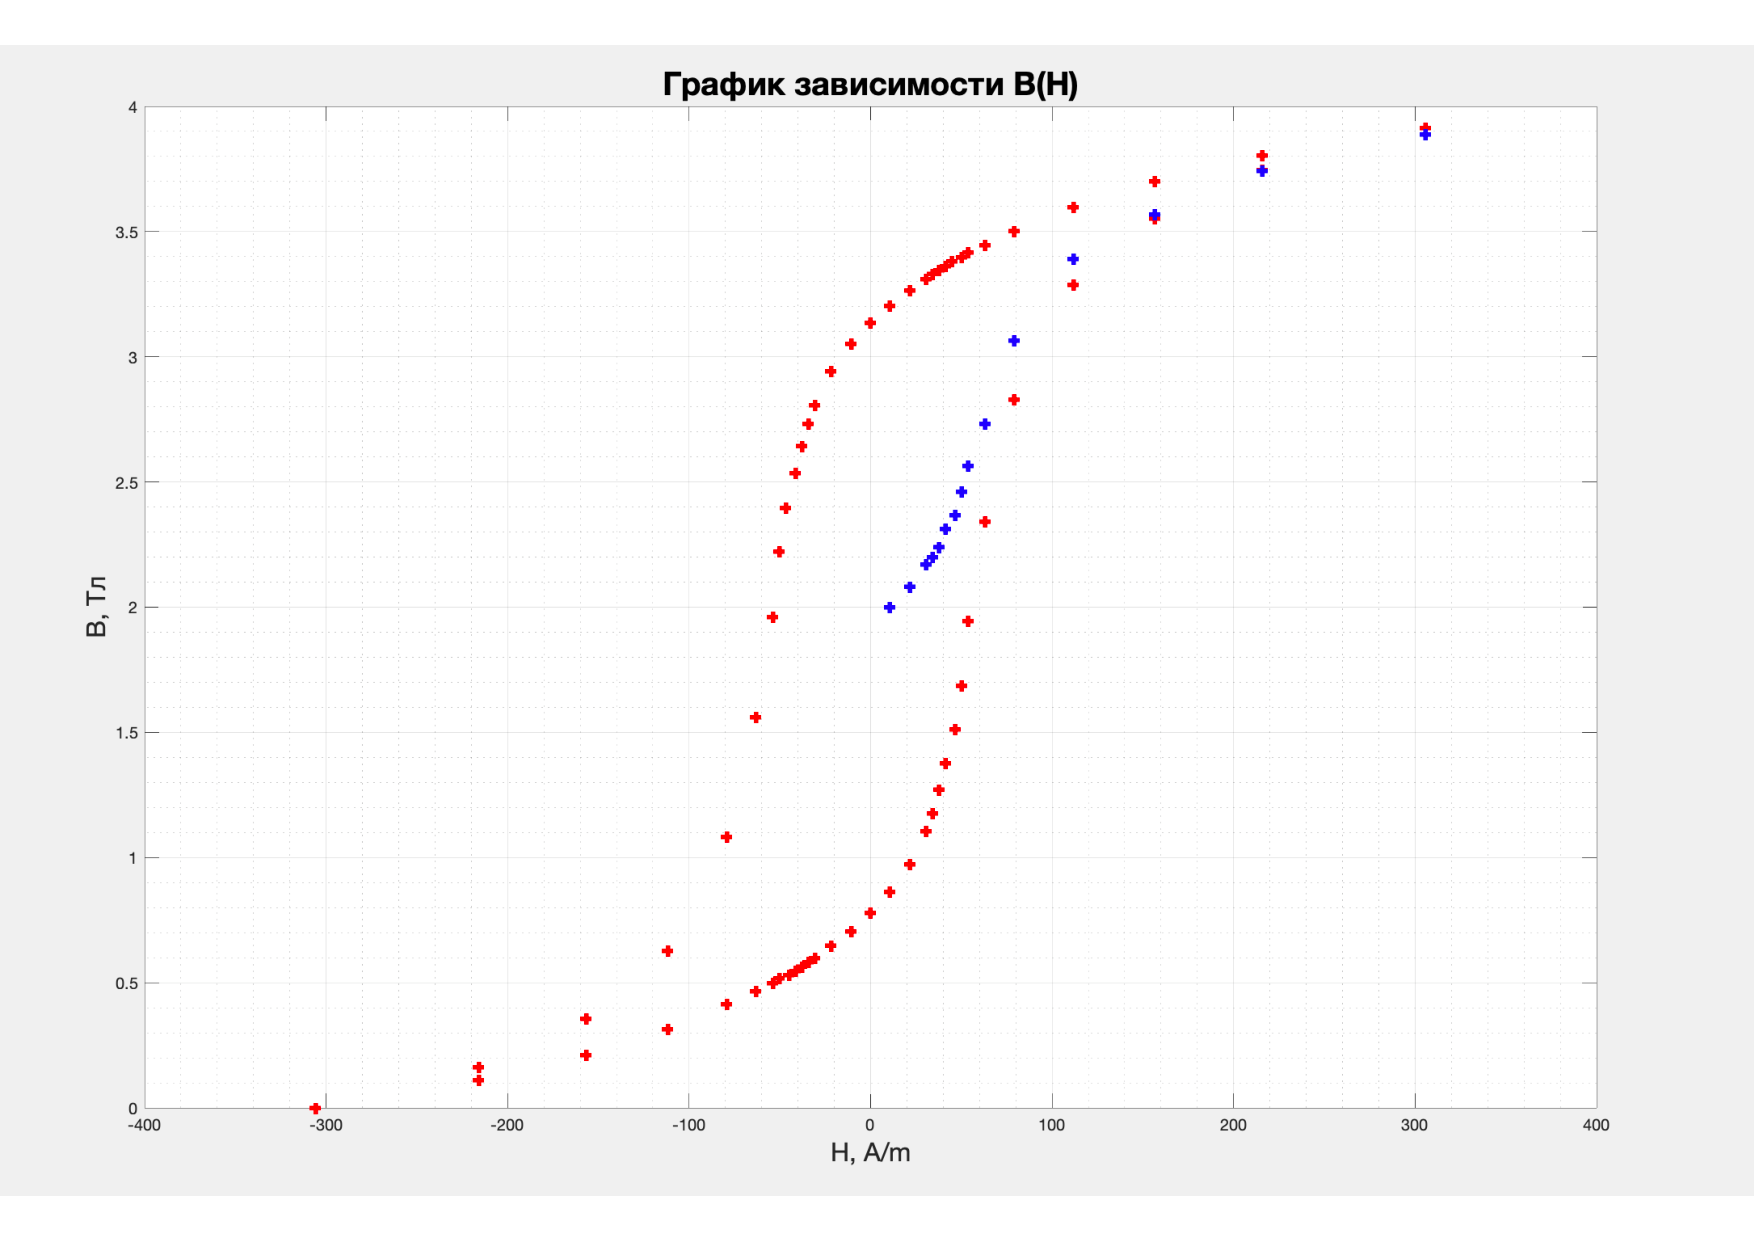
\includegraphics[width=\linewidth]{gra1.pdf}
	\caption{петля гистерезиса и кривая намагничивания}
	\label{gr1}
\end{figure}
\end{center}

По графику определяем значения:
\begin{itemize}
\item коэрцитивной силы $H_c = (54 \ \pm \ 2) \dfrac{\text{А}}{\text{м}}$
\item значение индукции насыщения $B_s = (1.89 \ \pm \ 0.05) \text{Тл}$
\item максимальное значение дифференциальной магнитной проницаемости $\mu_\text{диф} = \dfrac{1}{\mu_0} \dfrac{dB}{dH} = 4500 \pm 1300$
\end{itemize}

Табличные значения (взяты из справочника в пособии к лабораторным работам для технической стали): \[
H_c = 80 \ \dfrac{\text{А}}{\text{м}}, \ \ \
B_s = 2.15 \ \text{Тл}, \ \ \
\mu_\text{диф} = 5000. \ \ \
\]


\section*{Выводы}

\begin{enumerate}
	\item В ходе работы были исследованы петля гистерезиса магнитомягкого материала, его начальная кривая намагничивания.
	\item По кривой гистерезиса видно, что материал является магнитомягким, так как площадь петли мала. Также она симметрична и в целом соответствует теоретическим изображениям подобных кривых.
	\item Различие справочных и экспериментальных данных может объясняться тем, что, скорее всего, образец изготовлен не из чисто технического железа, а из сплава его с другим металлом.
\end{enumerate}


\end{document}